\section{The real ratio of the rubidium isotopes}
\label{sec:ratio}
Now we calculate the ratio of each isotope by identifying the area under every peak. For that we are fitting the gaussian distribution for each peak of our data for the reference beam absorption spectrum. We take the current axis because for the ratio it does not matter which axis we use. Furthermore, we use the data that is freed from any trends (look fig. \ref{image:trendless}).Then the fitting function has the form of:
\begin{gather}
    y = a\cdot\exp(-\left(\frac{(x-b)}{\sqrt{2}c}\right)^2)
    \label{eq:gaussFit}
\end{gather}
$b$ is here the x-value of each peak that we have already obtained in table \ref{tab:identify}. We get with the curve_fit of scipy.optimize package from python:
\begin{center}
    \begin{tabular}{c | c c c}
        peak & a/V & b/mA & c/mA\\
        \hline
        1 &  -0.00539 & 119.4429 & 0.57669\\
        2 &  -0.01742 & 125.0267 & 0.52976\\
        3 &  -0.03085 & 131.8581 & 0.62443\\
        4 &  -0.01462 & 134.7829 & 0.74425\\
    \end{tabular}
    \captionof{table}{fitting data for each peak}
\end{center}
In figure \ref{image:gaussFit} is shown how each gaussian fit looks for each peak.\\
With the parameter we calculated above we are now able to determine the area under each curve of each peak with the following relation:
\begin{gather}
    \int^{\infty}_{-\infty}\exp(-k(x-\mu)^2)\,dx = \sqrt{\frac{\pi}{k}} \xrightarrow{\mu = b,~k = \frac{1}{2c^2}}\int^{\infty}_{-\infty}a\cdot\exp(-\left(\frac{(x-b)}{\sqrt{2}c}\right)^2) = a \sqrt{2\pi c^2}
\end{gather}
This expression gives us then the area as follows:
\begin{center}
    \begin{tabular}{c | c | c}
        peak & isotope & area/$1\cdot 10^{-6}$ W\\
        \hline
        1 & $^{87}Rb$ &  -7.79 \\
        2 & $^{85}Rb$ & -23.13 \\
        3 & $^{85}Rb$ & -48.29 \\
        4 & $^{87}Rb$ & -27.27 \\
    \end{tabular}
    \captionof{table}{area under the curve of each peak}
\end{center}
The area under the peaks is proportional to the amount of atoms of each isotope in the gas what gives us:
\begin{gather}
    ^{85}Rb = \frac{23.13+48.29}{7.79+23.13+48.29+27.27} = 0.671 \Rightarrow  {^{87}Rb} = 0.329
\end{gather}
Meaning that in our probe there is \SI{67.1}{\percent} $^{85}Rb$ and \SI{32.9}{\percent} $^{87}Rb$ which compared to the literature (\SI{72.2}{\percent} $^{85}Rb$ and \SI{27.8}{\percent} $^{87}Rb$) shows that the assumption from chapter \ref{sec:freeing} to take the intensity into account was correct.
\begin{center}
    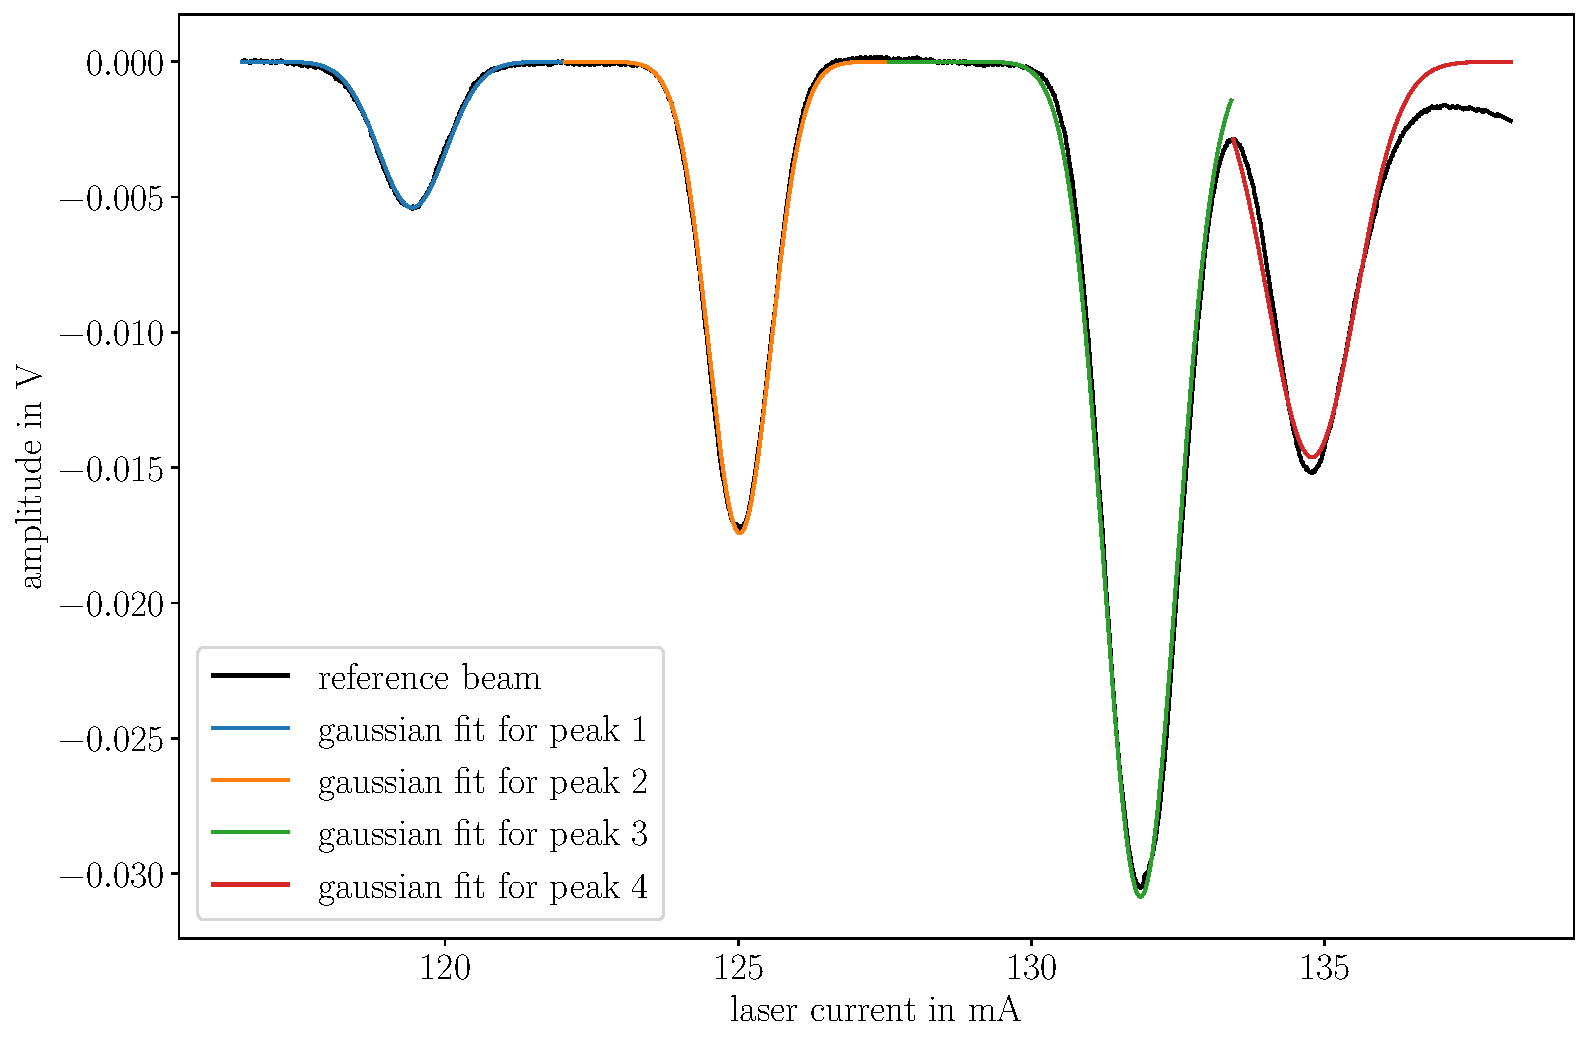
\includegraphics[scale=0.72, angle = 90]{Aufg-3/gaussFit.pdf}
    \captionof{figure}{gaussian fit for each Peak of the reference beam spectrum}
    \label{image:gaussFit}
\end{center}